% !TEX root = ./abstract.tex
% @Author: Xiaocheng Tang
% @Date:   2017-05-11 22:04:57
% @Last Modified by:   Xiaocheng Tang
% @Last Modified time: 2017-05-17 23:23:01

\begin{figure*}[th]
\centering
\begin{subfigure}[b]{0.35\textwidth}
   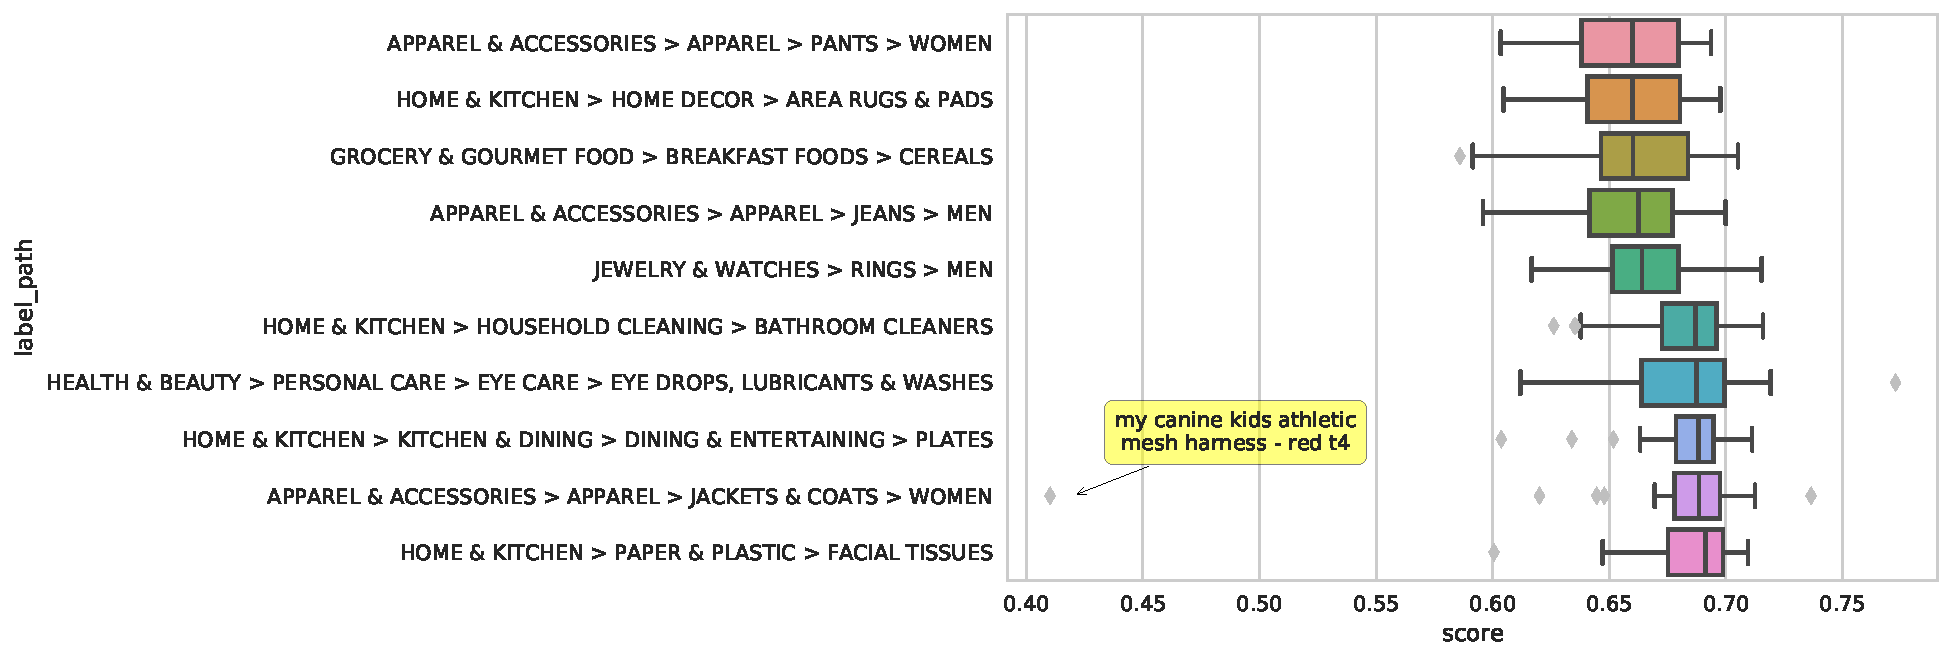
\includegraphics[width=\textwidth]{resources/noise-detect}
   \caption{Noisy training sample detection.  }
   \label{fig:noise-detect}
\end{subfigure}
\begin{subfigure}[b]{0.33\textwidth}
   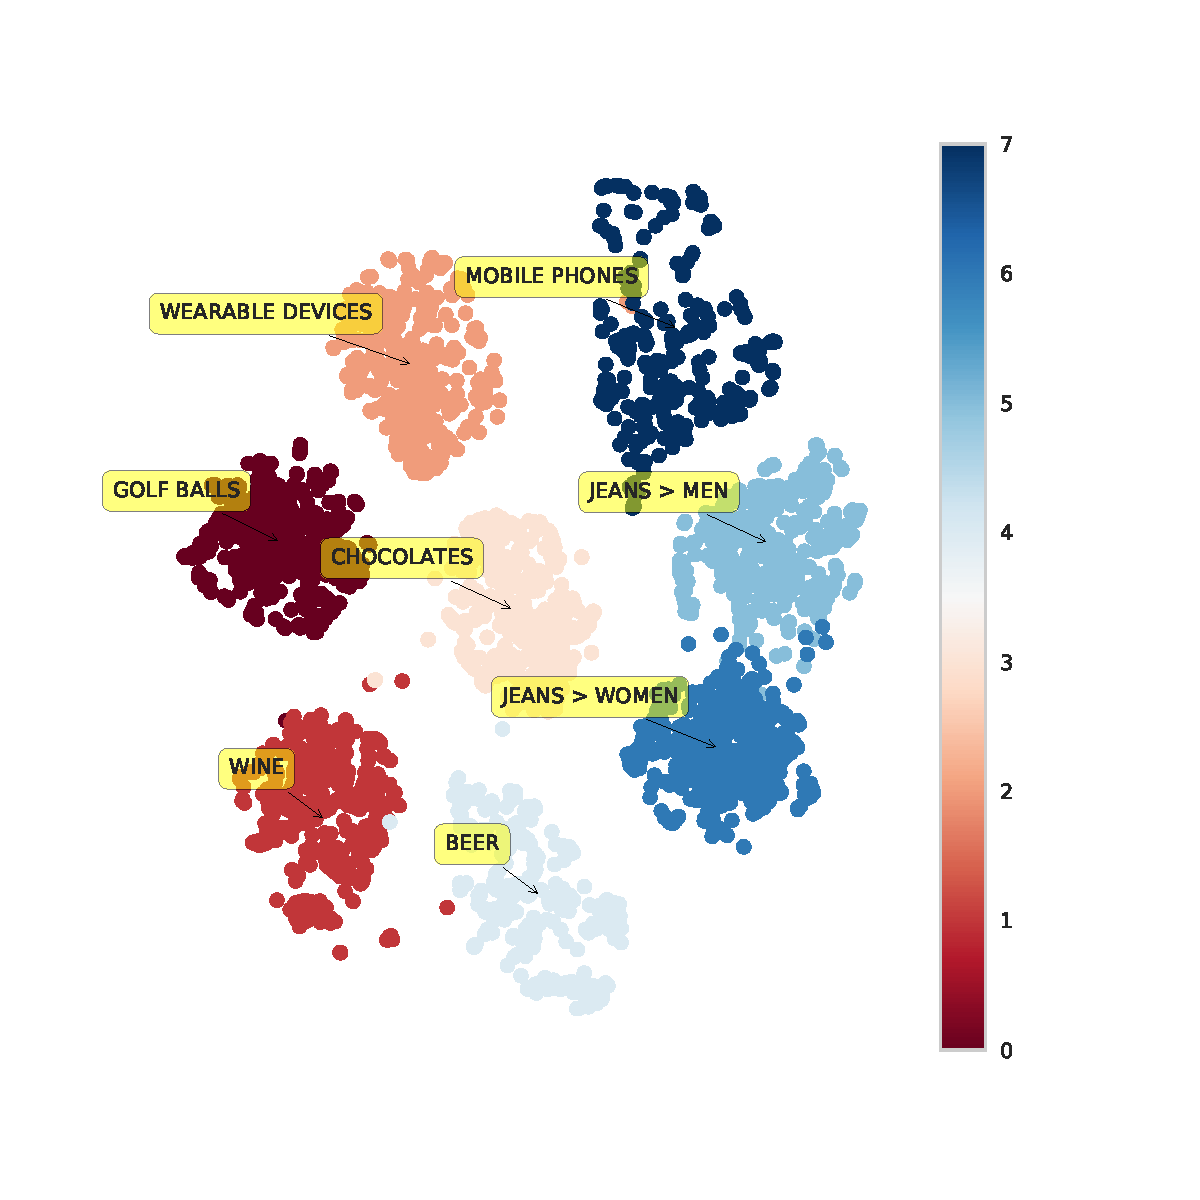
\includegraphics[width=\textwidth]{resources/cluster}
   \caption{Visualizations of item vector clusters.  }
   \label{fig:cluster}
\end{subfigure}
\begin{subfigure}[b]{0.3\textwidth}
   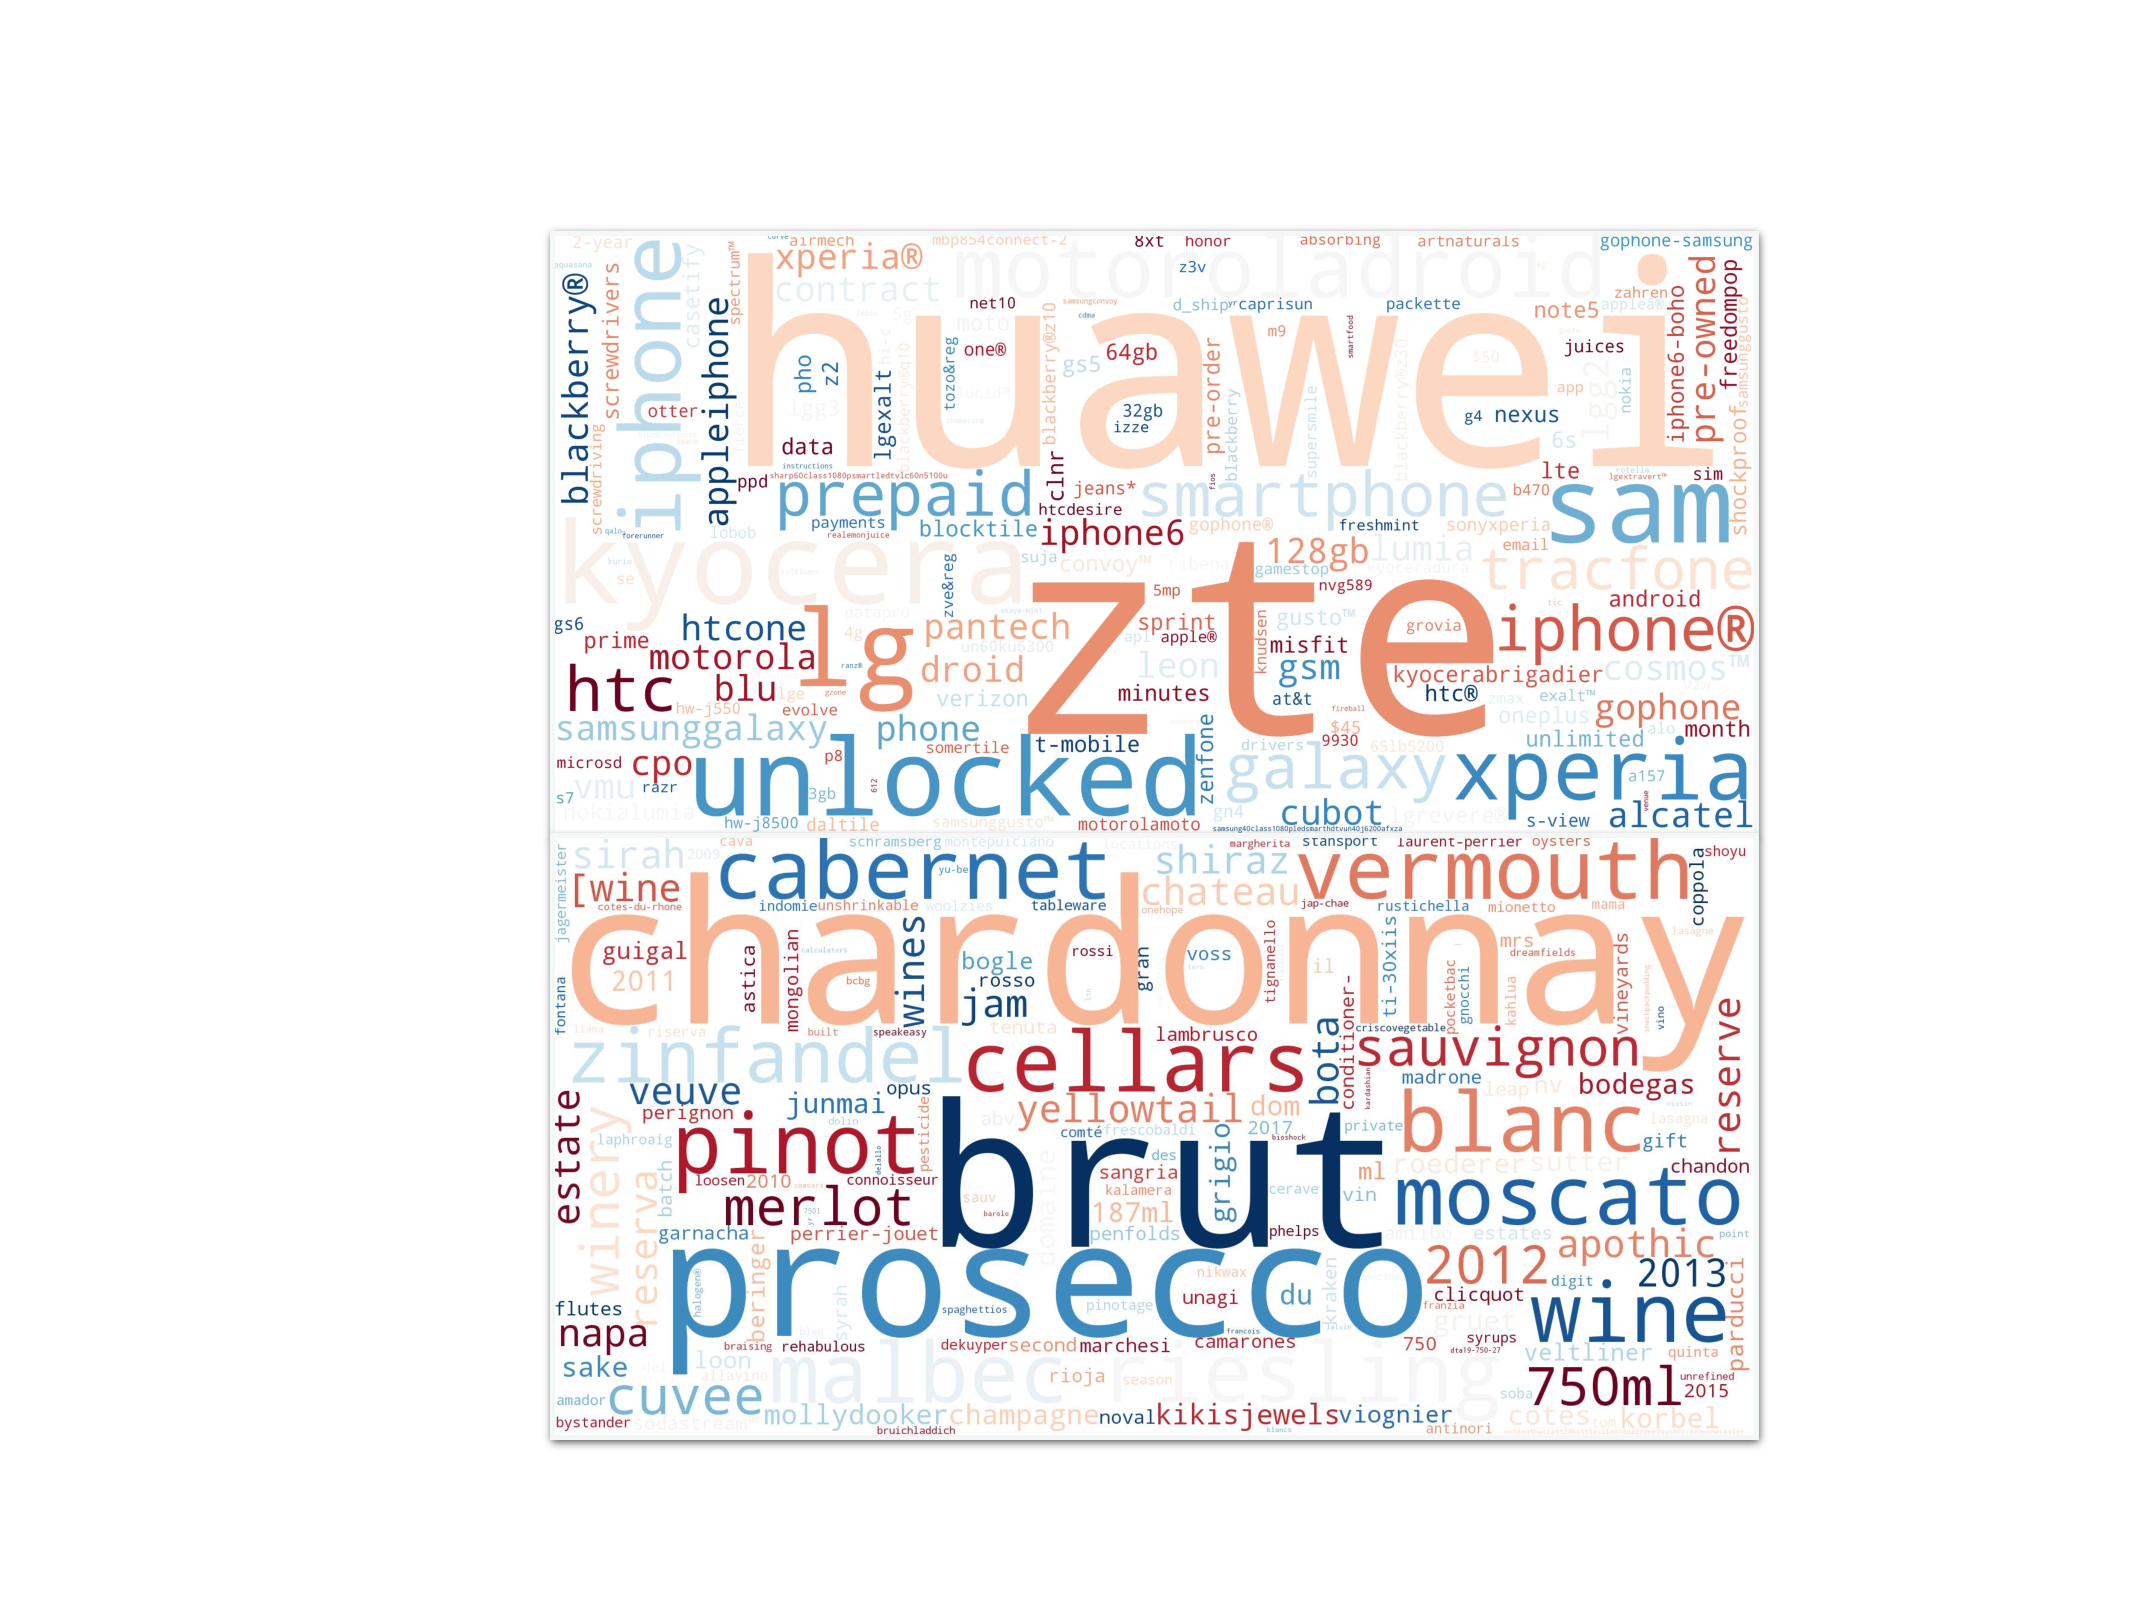
\includegraphics[width=\textwidth]{resources/wc}
   \caption{Top feature clouds.}
   \label{fig:wc}
\end{subfigure}
\caption{In (\ref{fig:noise-detect}) it shows eight categories and their training sample `confidence' scores distribution. Outliers are denoted by black dots. (\ref{fig:cluster}) visualizes the dense 50-dimensional item vectors that are projected onto the 2-dimensional space using t-SNE with 50 perplexity and PCA initialization. (\ref{fig:wc}) is generated from top key words in categories \emph{wine} (bottom) and \emph{mobile phones} (above). Words with bigger sizes indicate stronger predicators for the category.}
\end{figure*}

\subsection{De-noising Training Set} % (fold)
\label{sub:de_noising_training_sample}

Items with incorrect labels will affect the qualities of the categorization system if many are present in the dataset used for training. Those noisy items get introduced into the training set either due to conflict in the business rules or because of the labeling process which is often labor-intensive and error-prone. Here we use a de-noising approach based on active learning \cite{culotta2005reducing}, by alternatingly updating the least `confident' items given the classifier and the classifier given the training data. We observe that de-noising helps improve the accuracy of the system.
The main procedures are described in Algorithm \ref{alg:denoising}. 
An illustration of the intermediate results from one iteration of Algorithm \ref{alg:denoising} is shown in Figure~\ref{fig:noise-detect}. The training data confidence scores for nine categories are presented. 
Outliers are shown as black dots, for example, the obvious one at the left bottom corner of Figure~\ref{fig:noise-detect}. The central rectangle contains the scores between the first and the third quantile. A thin rectangle with high median score indicates a goodness of fit.
In the experiments we find that the outliers are either labeled incorrectly or the classifier failing to learn the item sufficiently. For the former we either relabel or remove them from the training set. and for the latter we duplicate and add them back to the training set to increase their exposures to the training algorithm so the system learn them better. 


\begin{algorithm2e}[htb]
\caption{Training Set De-noising Procedures.}
\label{alg:denoising}
  \textbf{Input}: $\XCal_o = \emptyset, \DCal = \XCal \times \CCal, U, V, \eta > 0$ \\ 
  \Repeat{$\XCal_o \neq \emptyset$}{
    retrain $U, V$ from $\DCal$ \\
    compute the logit matrix $L = XUV^T, L \in \Rmbb^{N \times |\CCal|}$ \\
    normalize $L$ such that all entries are between $(0, 1)$ \\
    create the vector $l \in \Rmbb^N$ where $l_i = L_{ic_i}$  \\
    set $\XCal_o$ to be empty \\
    \For{each $c \in \CCal$} {
        rank $l_c \in \Rmbb^{N_c}$ in descending order \\
        compute the range of variation ($IQR$) from $l_c$ \\
        collect points that are $\eta \times IQR$ below the first quantile \\
        add those points to $\XCal_o$
    }
    update $\DCal$ by either removing or relabeling $x \in \XCal_o$
  }
  \textbf{Output}: $U, V, \DCal$
\end{algorithm2e}

\subsection{Feature Representation And Selection} % (fold)
\label{sub:catefeature_selection}
We demonstrate that our end-to-end system does not require feature engineering or preprocessing in the sense that it automatically extracts and selects important features from raw item descriptions. Furthermore, it does not require the removal of stop words or punctuations. On the contrary, it is observed that using raw text without preprocessing improves the performance. Table~\ref{tab:features} shows the different features selected by different categories for prediction. The features are ranked by their relative importance to the given category vector. The importance scores are obtained by taking the inverse of the cosine distance between the category and the feature in the vector space. Notice that many world-famous brands are selected as important features, such as levi's for \emph{jeans}, fitbit, jawbone for \emph{wearable devices}, and ferrero, hersheys for \emph{chocolates}, etc. This makes sense since those brand words might very well be the most frequent words in that category. However, notice also that no stop words make it to the list although they are quite frequent as well. Moreover, note that each category automatically selects its own set of features for prediction, although features are shared among all categories. For example, it is interesting to see that the system figures out on its own that, for jeans, 501 is more popular with men while women like 524. Finally Figure~\ref{fig:cluster} demonstrates the discriminative property of the item vectors. In this experiment, we take a subset of items from eight categories and project them onto the 2-dimensional space. It can be seen from the figure that eight clusters are easily identified and well separated. It is interesting to notice that categories with similar meaning are close to each other, e.g., electronic devices (wearable and phones) on the top and apparel (men and women jeans) on the right side.  
% subsection catefeature_selection (end)



% subsection de_noising_training_sample (end)

\begin{table*}
  \caption{Strongest Unigram Signals / Keywords for Category Prediction}
  \label{tab:features}
  \begin{tabular}{cccccccl}
    \toprule
    JEANS > MEN	&	JEANS > WOMEN	&	WEARABLE DEVICES	&	 BEER	&	 WINE	&	CHOCOLATES	&	 GOLF BALLS	 & MOBILE PHONES \\
    \midrule
    brixton	&	jeans-	&	smartwatch	&	ipa	&	chardonnay	&	ferrero	&	titleist	&	zte	\\
    graduate	&	suki	&	misfit	&	ale	&	brut	&	m\&m	&	srixon	&	huawei	\\
    normandie	&	super-skinny	&	fitbit	&	beer	&	prosecco	&	lindt	&	callaway	&	kyocera	\\
    fit-	&	rips	&	jawbone	&	budweiser	&	riesling	&	hersheys	&	maxfli	&	unlocked	\\
    rude	&	wedgie	&	forerunner	&	lagunitas	&	pinot	&	m\&ms	&	volvik	&	sam	\\
    skinny-fit	&	straight-leg &	vivofit	&	heineken	&	malbec	&	milka	&	taylormade	&	lg	\\
    levi's\textregistered	&	pajamajeans	&	tracker	&	coors	&	cellars	&	snickers	&	pinnacle	&	xperia	\\
    501	&	stevie	&	fitness	&	lager	&	wine	&	kisses	&	bridgestone	&	iphone	\\
    a\&f	&	524\texttrademark	&	nike+	&	modelo	&	vermouth	&	kinder	&	balls	&	motoroladroid	\\
    527	&	524	&	pebble	&	shiner	&	moscato	&	cadbury	&	dozen	&	smartphone	\\
    sartor	&	5pkt	&	garmin	&	peroni	&	blanc	&	ghirardelli	&	distance	&	 iphone\textregistered	\\
    selvedge	&	jegg	&	withings	&	bottles	&	cabernet	&	brookside	&	wilson	&	galaxy	\\
    carpenter	&	rockstar	&	vivosmart	&	guinness	&	zinfandel	&	twix	&	golf	&	htc	\\
    stonewash	&	nouveau	&	activity	&	corona	&	sauvignon	&	butterfinger	&	cornmeal	&	prepaid	\\
    matchbox	&	seabreeze	&	smartband	&	sixpoint	&	750ml	&	godiva	&	flite	&	tracfone \\
    \bottomrule
  \end{tabular}
\end{table*}


\subsection{Rule Integration} % (fold)
\label{sub:rule-integration}

We conducted the experiments for six categories listed in Table (\ref{tab:numrules}). Since current implementation
of generative model is binary(\cite(link to snorkel)), we applied it to each category separately and combined the results in a final output.

The generative model outputs marginal probabilites for each product item. Figure (\ref{fig:genmodel_pred_probs}) demonstrates
the distribution of those probabilities for some categories.
We assume that the product belongs to certain category if prediction probability is greater or equal to 0.5.

In addition, we demonstrate the fraction of coverage, overlaps and conflicts in Figure (\ref{fig:covconflict}). The diagram shows
 small rule coverage and the presence of conflicts and overlaps in 'Boots \textgreater Men' category.

We used unlabeled product items to train generative model and applied learned model to manually label test data and measure
prediction accuracy. The train and test sets contain respectively 100k and 20k product items. According to
our experimental results shown in table (\ref{tab:evaluation}), 'Boots \textgreater Women' category has high precision/recall and accuracy due to
precise and less conflictous rules, whereas 'Boots \textgreater Men' category has less rules but more overlaps and conflicts.
High accuracy score in 'Men \greater Boots' category is associated with the large number of true negatives which overly exceeds
true/false positives and false negatives in that category.

Ultimately, we combine generated and manually labeled training sets to train a discriminative model to predict accurate product categories.

\begin{table*}
  \caption{Examples of the category labels and the total numbers of rules in each category}
  \label{tab:numrules}
  \begin{tabular}{ll}
    \toprule
    Category & \#Rules\\
    \midrule
    Boots \textgreater Women &  88  \\
    Boots \textgreater Men  & 36 \\
    Travel \textgreater Hotel & 30 \\
    Home \textgreater LampShades & 19 \\
    Home \textgreater Other & 11 \\
    Grocery \textgreater Nutrition Drinks & 11 \\
    \bottomrule
  \end{tabular}
\end{table*}

\begin{table*}
  \caption{Evaluation results for several categories on sub-sampled data}
  \label{tab:evaluation}
  \begin{tabular}{lllllll}
    \toprule
    Category & Presicion & Recall & F1 & Accuraccy & Neg Class Accuracy & Pos Class Accuracy\\
    \midrule
    Boots \textgreater Women  & 93\% & 96\% & 94\% & 99\% & 96\% & 93\% \\
    Boots \textgreater Men &  60\%  & 75\% & 66\% & 99\% & 75\% & 60\% \\
    \bottomrule
  \end{tabular}
\end{table*}

\begin{figure}[th]
   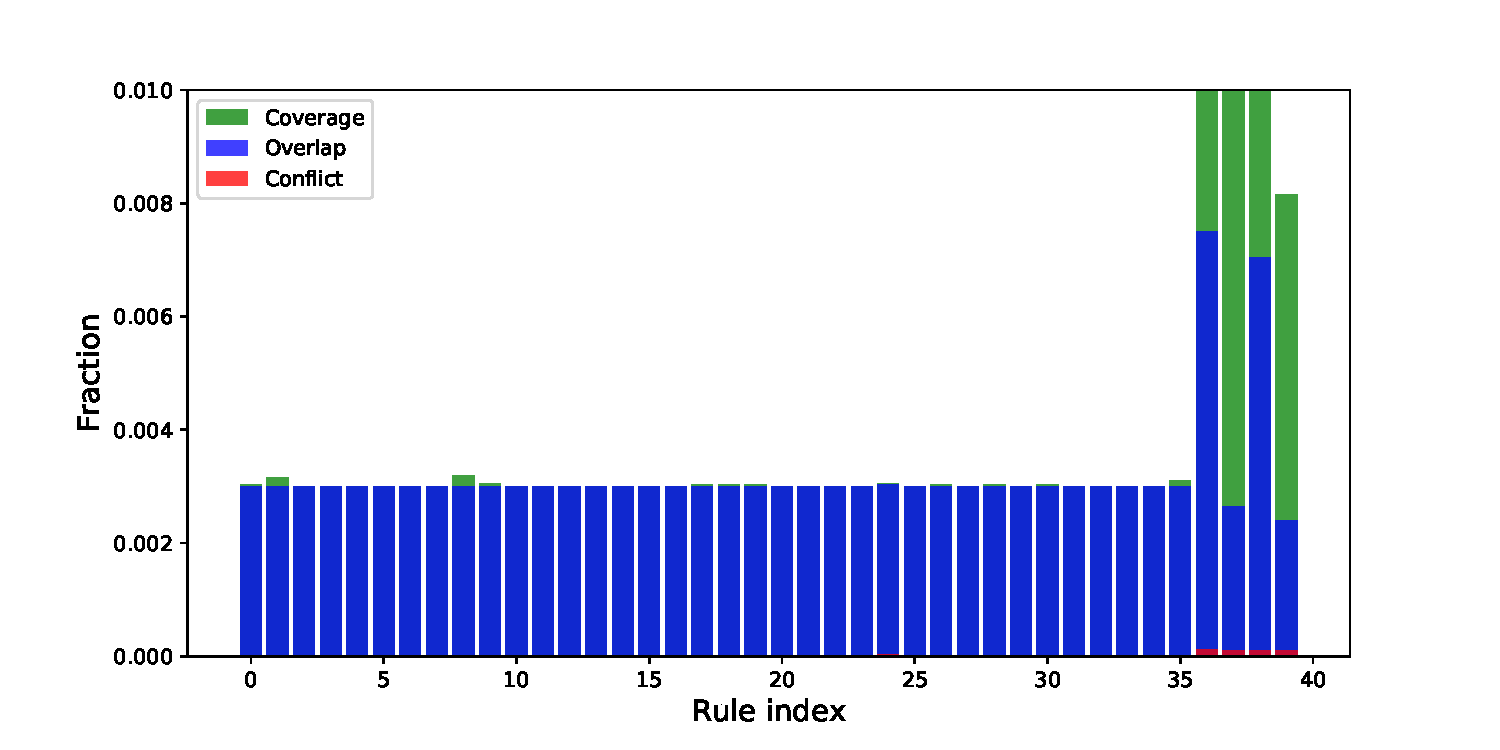
\includegraphics[width=0.5\textwidth]{resources/covconflict}
   \caption{The fraction of coverage, overlaps and conflicts for the rules from 'Boots \textgreater Men' category}
   \label{fig:covconflict}
   \centering
\end{figure}
\begin{figure}[th]
   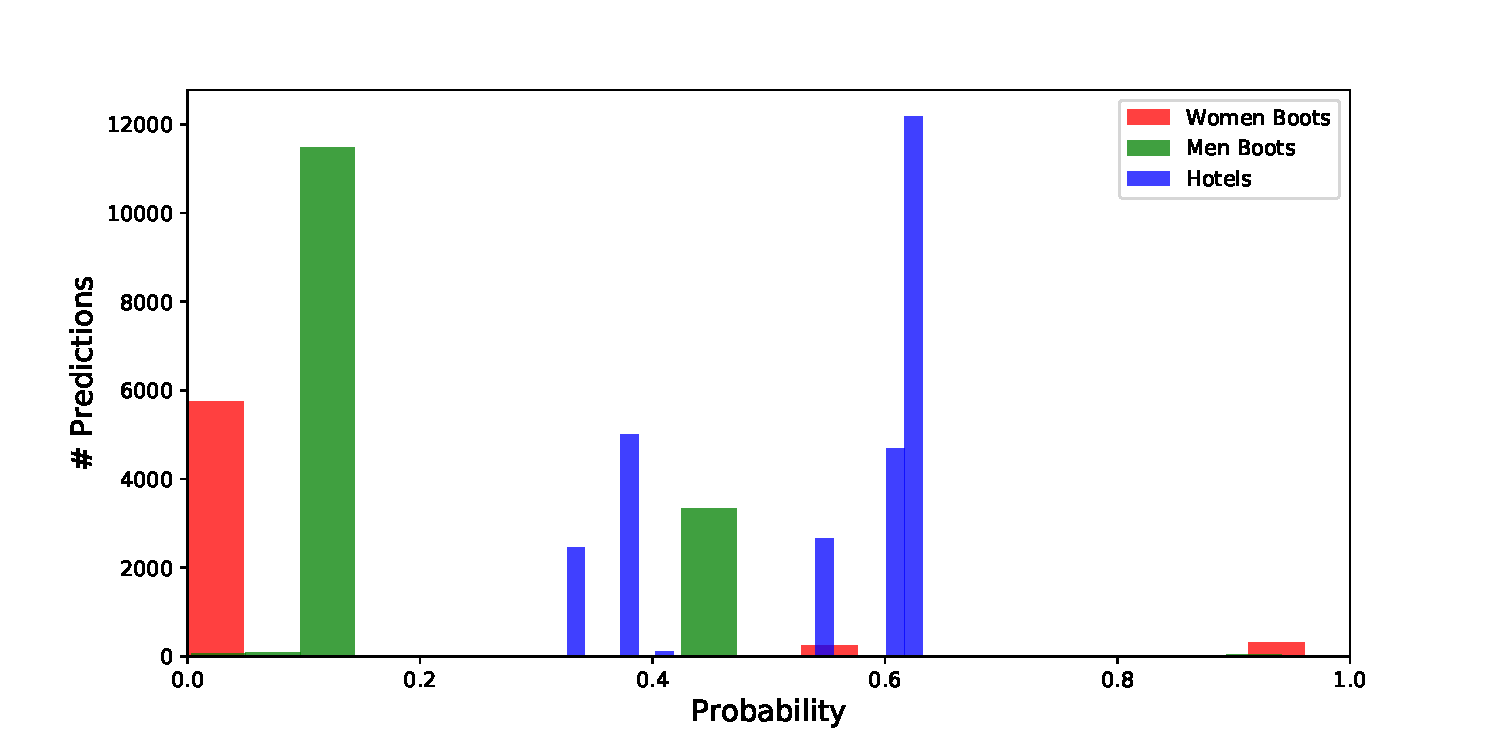
\includegraphics[width=0.5\textwidth]{resources/genmodel_pred_probs}
   \caption{The distribution of marginal probabilities}
   \label{fig:genmodel_pred_probs}
   \centering
\end{figure}

